\newpage
\begin{song}{title={Morze, moje morze}, music={EKT Gdynia}}
    \begin{intro}
        \writechord{d} \writechord{g} \writechord{F} \writechord{A7} \\
        \writechord{d} \writechord{g} \writechord{A7} \writechord{d}
    \end{intro}
    \begin{multicols}{2}
    \begin{verse}
        ^{d}Hej, me Bał^{A7}tyckie Mo^{d}rze ^{C} \\
        W^{F}dzięczny ci ^{C}jestem bar^{F}dzo \\
        |: ^{g}Toś ty mnie ^{C}wychowało \\
        ^{F} Toś ty mnie ^{g}wychowało \\
        Sz^{d}kołęś mi ^{A}dało twar^{d}dą :|
    \end{verse}
    \begin{verse}
        Szkołęś mi dało twardą \\
        Uczyłoś łodzą pływać \\
        Żagle pięknie cerować, \\
        Żagle pięknie cerować, \\
        Codziennie pokład zmywać
    \end{verse}
    \begin{verse}
        Codziennie pokład zmywać \\
        Od soli i od kurzy \\
        Mosiądze wyglansować \\
        Mosiądze wyglansować \\
        W ciszy, czy w czasie burzy
    \end{verse}
    \begin{center}
        \vspace{0.6cm}
        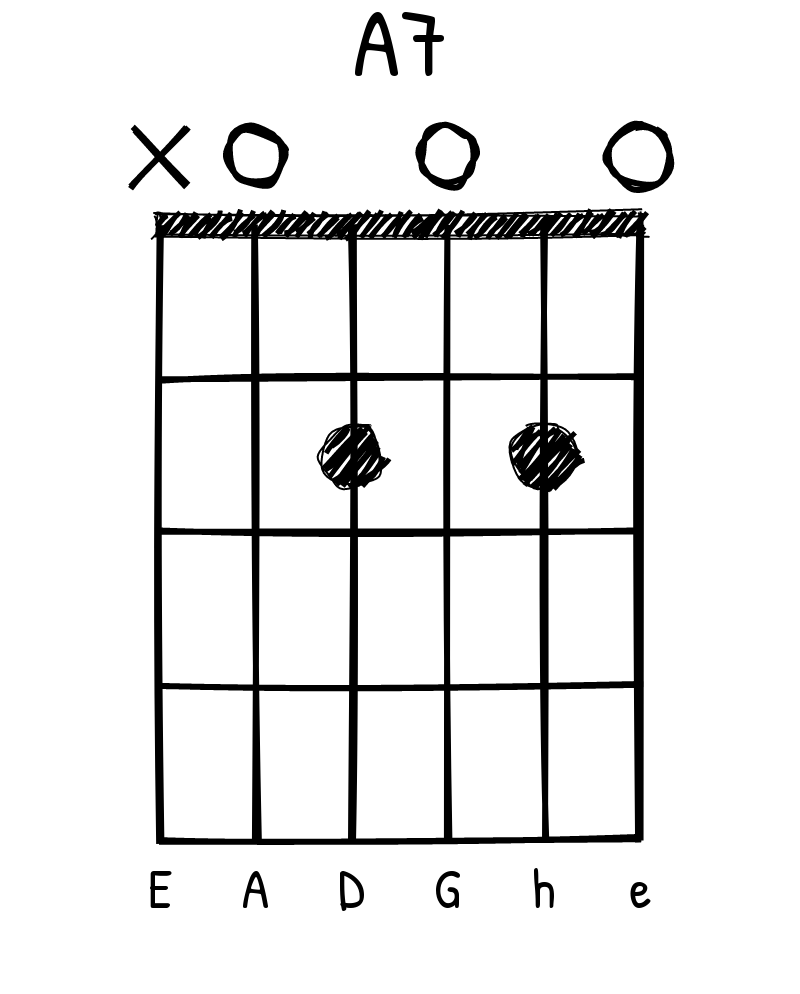
\includegraphics[height=3.5cm]{images/A7.png}
    \end{center}
    \vfill\null\columnbreak{}
    \begin{verse}
        W ciszy, czy w czasie burzy \\
        Trzeba przy pracy śpiewać \\
        Bo kiedy śpiewu nie ma \\
        Bo kiedy śpiewu nie ma \\
        Neptun się będzie gniewać
    \end{verse}
    \begin{verse}
        Neptun się będzie gniewać \\
        I klątwę brzydką rzuci \\
        Wpakuje na mieliznę \\
        Wpakuje na mieliznę \\
        Albo nam łódź wywróci
    \end{verse}
    \begin{verse}
        Albo nam łódź wywróci \\
        I krzyknie: \say{Hej, partacze! \\
        Nakarmię wami rybki \\
        Nakarmię wami rybki \\
        Nikt po was nie zapłacze!}
    \end{verse}
    \begin{verse}
        Nikt po nas nie zapłacze \\
        Nikt nam nie dopomoże \\
        Za wszystkie miłe rady \\
        Za wszystkie miłe rady \\
        Dziękuję tobie, Morze
    \end{verse}
    \begin{verse}
        Hej, Morze, moje Morze \\
        Wdzięczny ci jestem bardzo \\
        Toś ty mnie wychowało \\
        Toś ty mnie wychowało \\
        Szkołęś mi dało twardą
    \end{verse}
    \end{multicols}
\end{song}

